\documentclass{article}

\usepackage{amsmath}
\usepackage{amssymb}
\usepackage{graphicx}
\usepackage{tikz}
\usetikzlibrary{arrows}
\usepackage{verbatim}
\usepackage{sfmath}
\usepackage{psfrag}
\usepackage{here} 
\usepackage{hyperref}
\usepackage{xcolor}
\usepackage{tcolorbox}


\renewcommand{\familydefault}{\sfdefault}
\renewcommand{\familydefault}{cmss}

\begin{document}

\begin{center}
\bf{\huge 
Ingenier\'{\i}a de Control\\
\vspace{0.25cm}
Problem 1
}
\end{center}

\section*{Aircraft vertical takeoff and landing}

Consider the simplified planar model of the system for vertical takeoff and landing of an aircraft represented in Figure~\ref{fig:figure_1}, in which the aircraft is represented by a bar. 
The position of the center of mass of the aircraft, $\mathbf{c} =  (x, y)^T$, the roll angle of the aircraft, $\theta$, and their time derivatives are the state variables of the system.  
The thrust force $S$, applied to the center of mass of the aircraft, and the forces $F$, applied to the wing tips, are the control inputs $u_1$ and $u_2$ of the system, respectively.
The thrust force $S$ keeps the aircraft flying.
The forces $F$, which always act in opposite directions, control the roll of the aircraft.  



\begin{figure}[H]
\centerline{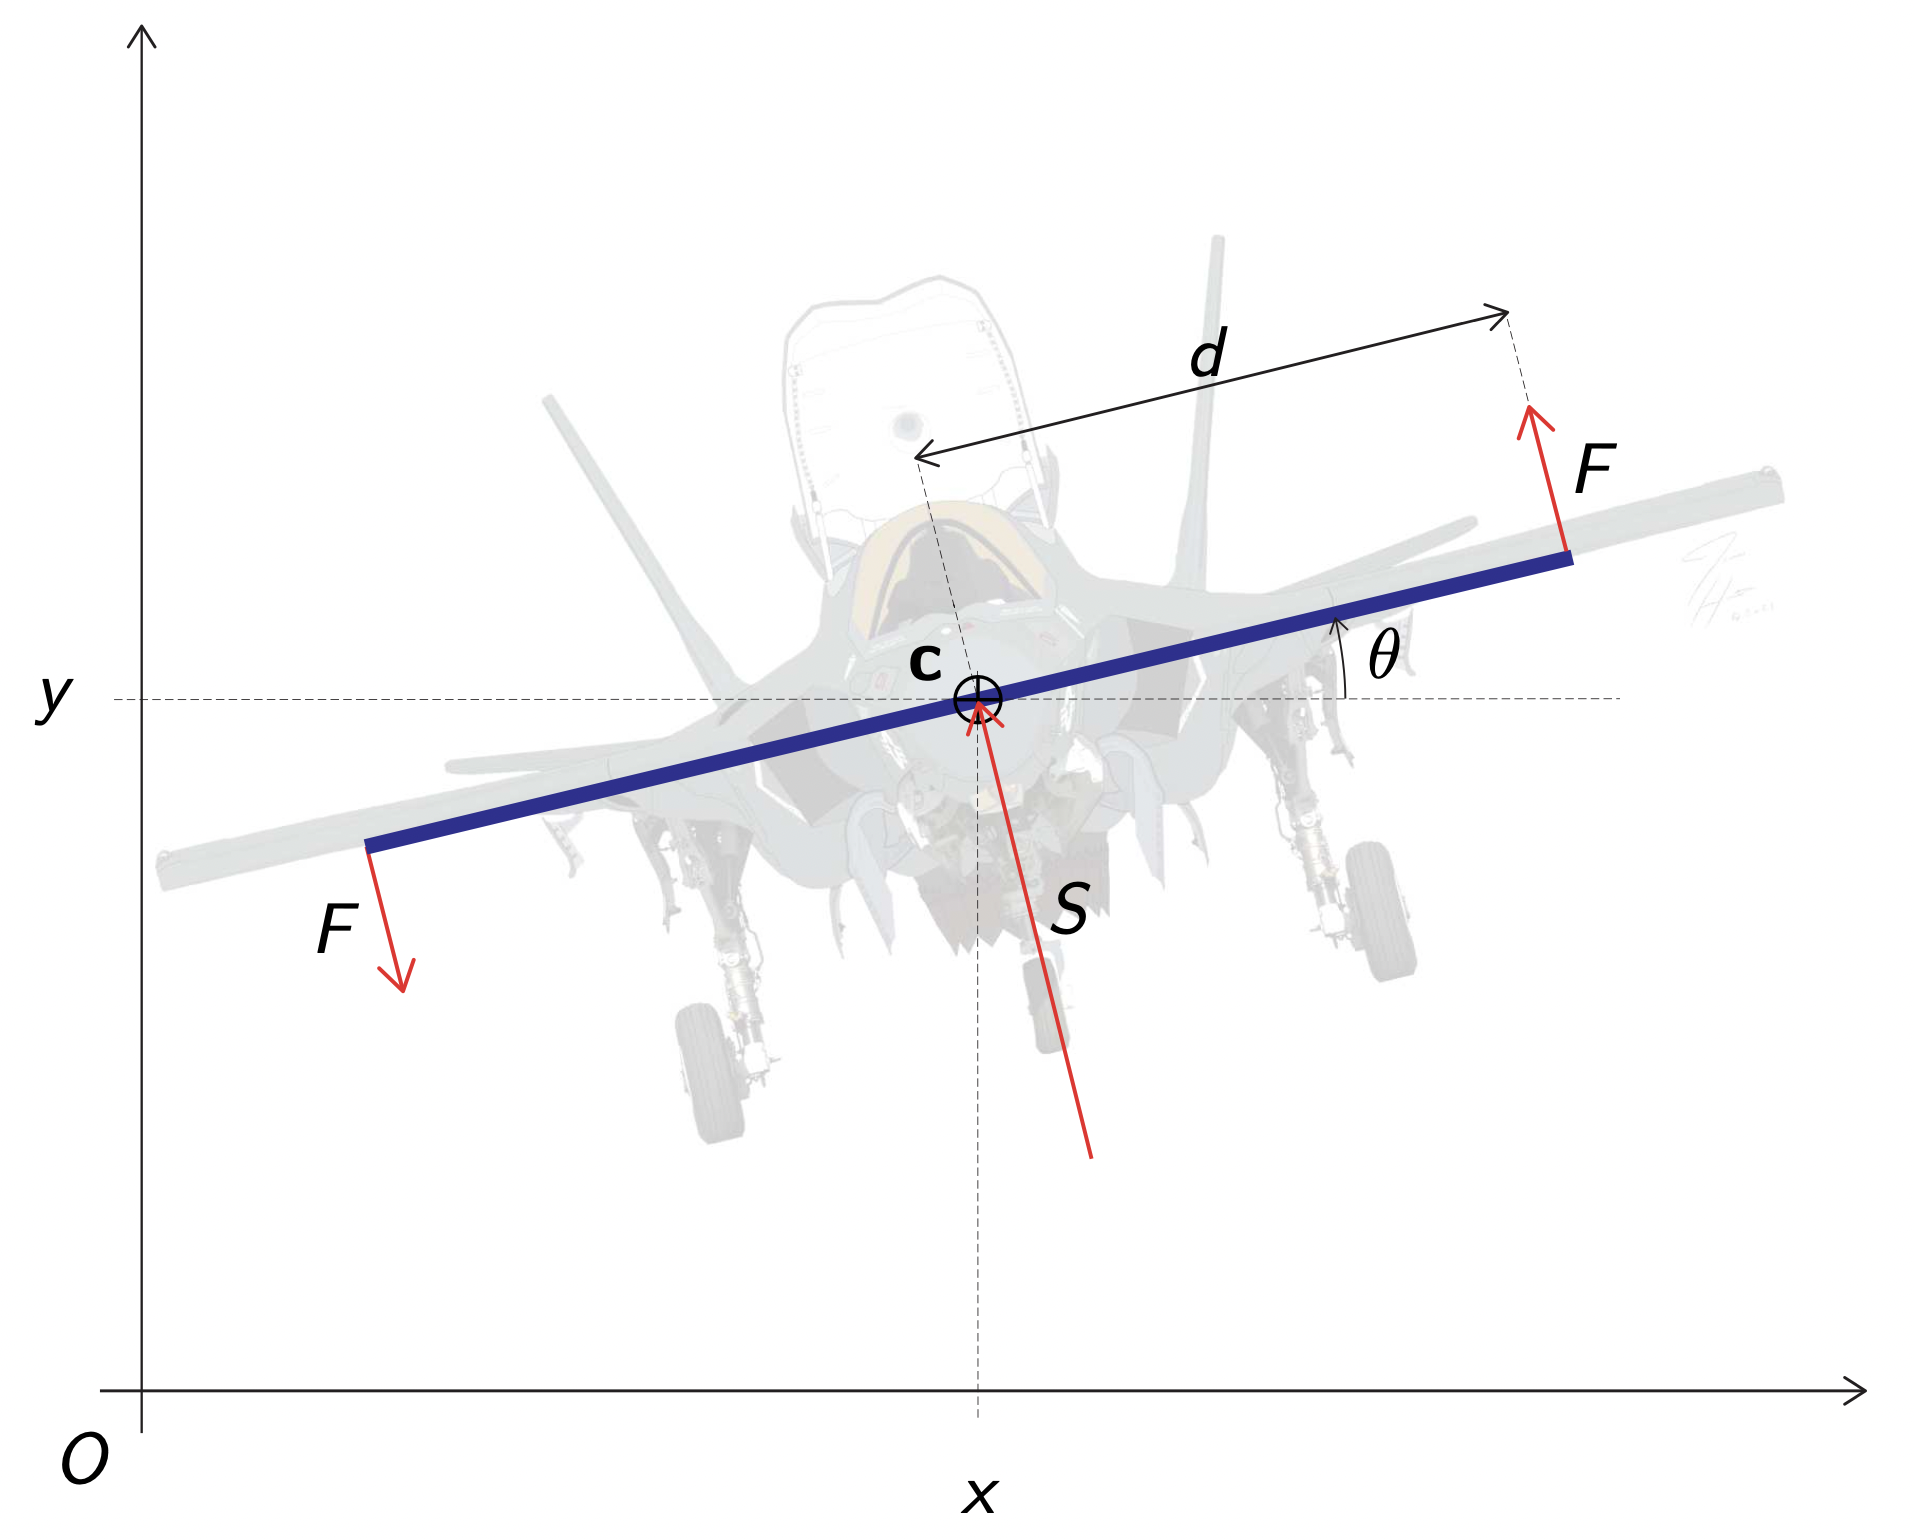
\includegraphics[width=0.75\columnwidth]{drawing}}
\caption{Sketch of the system for aircraft vertical takeoff and landing.}
\label{fig:figure_1}
\end{figure}


\noindent
The dynamic model of this system is
\begin{eqnarray*}
\ddot{x}  &=&- \frac{1}{m}  \sin (\theta) S,\\
\ddot{y} &=&- g + \frac{1}{m} \cos ( \theta) S, \\
 \ddot{\theta} &=& \frac{2 d}{J}  F,
\end{eqnarray*}
with the following parameters 
\begin{itemize}
\item
barycentric moment of inertia of the aircraft: $J = 10 000 \; [\text{kg m}^2]$, 
\item
mass of the aircraft: $m = 30 000 \; [\text{kg}]$, 
\item
$d = 5.5 \; [\text{m}]$, 
\item
gravity acceleration: $g = 9.81 \; [\text{m}/\text{s}^2]$.
\end{itemize}


















\begin{itemize}

\item[1)] Demonstrate the equations of the dynamic model using the Lagrange method.

\item[2)] Calculate the state space representation of the system, assuming that $\mathbf{x} = (x, y, \theta, \dot{x}, \dot{y}, \dot{\theta})^T = ( x_1, x_2, x_3, x_4, x_5, x_6)^T$, where distances are measured in [m], angles in [rad], linear velocities in [m/s], and angular velocities in [rad/s].

\end{itemize}


\bigskip

\noindent
\textcolor{red}{Write a detailed report answering each question in a different section. Originality and completeness of the answers will be the aspects that will be taken into account in the grading of the report. 
} 


\section*{Solution}


\begin{itemize}

\item[1)] {\color{gray} Demonstrate the equations of the dynamic model using the Lagrange method.}

Mediante el metodo de Lagrange hallamos las ecuaciones de estado del modelo dinamico, sabiendo que: L = T - V\\\\
		$L = \frac{1}{2}(m(\dot{x}^2+\dot{y}^2)+J\dot{\theta}^2) - mgy$\\

Por tanto, las ecuaciones de Lagrange son las siguientes:\\\\
		$\frac{d}{dt}\frac{\partial L}{\partial \dot{x}} - \frac{\partial L}{\partial x} = S$\\\\
		$\frac{d}{dt}\frac{\partial L}{\partial \dot{y}} - \frac{\partial L}{\partial y} = S$\\\\
		$\frac{d}{dt}\frac{\partial L}{\partial \dot{\theta}} - \frac{\partial L}{\partial \theta} = F$\\\\

Tanto en la primera ecuacion como en la segunda, se iguala a la fuerza de empuje aplicada al centro de masas, mientras que en la tercera, se iguala a la fuerza aplicada en las puntas de las alas.\\

Resolvemos la primera ecuacion\\\\
		$\frac{\partial L}{\partial \dot{x}} = m\dot{x}$\\\\
		$\frac{d}{dt}\frac{\partial L}{\partial \dot{x}} = m\ddot{x}$\\\\
		$\frac{\partial L}{\partial x} = 0$\\\\
obteniendo la primera ecuacion de Lagrange:\\\\
		$m\ddot{x} = -S_x sen(\theta)$.\\

De la misma manera\\\\
		$\frac{\partial L}{\partial \dot{y}} = m\dot{y}$\\\\
		$\frac{d}{dt}\frac{\partial L}{\partial \dot{y}} = m\ddot{y}$\\\\
		$\frac{\partial L}{\partial y} = -mg$\\\\
obtenemos la segunda ecuacion de Lagrange: \\\\
		$m(\ddot{y} + g) = S_y cos(\theta)$.\\\\
Por último\\\\
		$\frac{\partial L}{\partial \dot{\theta}} = J\dot{\theta}$\\\\
		$\frac{d}{dt}\frac{\partial L}{\partial \dot{\theta}} = J\ddot{\theta}$\\\\
		$\frac{\partial L}{\partial \theta} = 0$\\\\
obtenemos la tecera y última ecuacion de Lagrange:\\\\
		$J\ddot{\theta} = F2d$.\\\\
En esta última multiplicamos la fuerza por 2d dado que es la distancia total entre la punta de una ala y la otra.\\\\Tal como podemos comprobar, dichas ecuaciones coinciden con las que teniamos que demostrar.

\item[2)] {\color{gray} Calculate the state space representation of the system, assuming that $\mathbf{x} = (x, y, \theta, \dot{x}, \dot{y}, \dot{\theta})^T = ( x_1, x_2, x_3, x_4, x_5, x_6)^T$, where distances are measured in [m], angles in [rad], linear velocities in [m/s], and angular velocities in [rad/s].}

Asumiendo que:\\\\
		$x = 
			\begin{pmatrix}
				 x_1\\x_2\\x_3\\x_4\\x_5\\x_6
			\end{pmatrix}
		 		= 
			\begin{pmatrix}
				 x\\y\\\theta\\\dot{x}\\\dot{y}\\\dot{\theta}
			\end{pmatrix}$,\\\\
podemos escribir:\\\\
		$\frac{d}{dt}
			\begin{pmatrix}
				 x\\y\\\theta\\\dot{x}\\\dot{y}\\\dot{\theta}
			\end{pmatrix}
				=
			\begin{pmatrix}
				 \dot{x}\\\dot{y}\\\dot{\theta}\\\ddot{x}\\\ddot{y}\\\ddot{\theta}
			\end{pmatrix}
				=
			\begin{pmatrix}
				 \dot{x}\\\dot{y}\\\dot{\theta}\\-\frac{1}{m}\sin(\theta)S_x\\-g+\frac{1}{m}\cos (\theta)S_y\\\frac{2d}{J}F
			\end{pmatrix}$.\\\\
Por tanto, la representacion del espacio de estados es:\\\\
	$\dot{x_1}=x_4$,\\
	$\dot{x_2}=x_5$,\\
	$\dot{x_3}=x_6$,\\
	$\dot{x_4}=-\frac{1}{m}\sin(\theta)S_x$,\\
	$\dot{x_5}=-g+\frac{1}{m}\cos (\theta)S_y$,\\
	$\dot{x_6}=\frac{2d}{J}F$\\	

\end{itemize}




\end{document}
